\documentclass[aspectratio=169]{beamer}
\usepackage{amsmath,amssymb,amsfonts}
\usepackage{tikz}
\usetheme{Madrid}
\usetikzlibrary{positioning,arrows.meta}

\title{\textbf{Set Theory, Relations and Inclusion--Exclusion}}
\author{GAYATHRI P S}
\date{\textit{13 AUG 2026}}

\begin{document}

\begin{frame}
\titlepage
\end{frame}

\begin{frame}{Contents}
\begin{enumerate}
\item Sets
\item Set-Builder Form and Roster Form
\item Types of Sets
\item Set Operations
\item Relations
\item Equivalence Relations
\item Partial Orders and Posets
\item Hasse Diagrams
\item General Principle of Inclusion--Exclusion
\end{enumerate}
\end{frame}

\begin{frame}{What is a Set?}
\begin{block}{Definition}
A \textbf{set} is a well-defined collection of distinct objects.
\end{block}

The objects in a set are called \textbf{elements} or \textbf{members} of the set.

For example,
\[
A=\{1,2,3,4,5\}.
\]

Here,
\[
1,2,3,4,5\in A.
\]

If $x$ does not belong to $A$, we write
\[
x\notin A.
\]
\end{frame}

\begin{frame}{Set-Builder Form}
\begin{block}{Definition}
Set-builder form describes a set by stating the property or condition satisfied by its elements.
\end{block}

It is generally written as
\[
A=\{x\mid P(x)\}.
\]

Example:
\[
A=\{x\mid x\in\mathbb{N},\ 1\leq x\leq5\}.
\]

This means that $A$ contains all natural numbers from 1 to 5.

Therefore,
\[
A=\{1,2,3,4,5\}.
\]
\end{frame}

\begin{frame}{Roster Form}
\begin{block}{Definition}
Roster form represents a set by listing all its elements inside braces.
\end{block}

Example:
\[
A=\{1,2,3,4,5\}.
\]

The same set can be written in set-builder form as
\[
A=\{x\mid x\in\mathbb{N},\ 1\leq x\leq5\}.
\]

Thus, set-builder form gives a \textbf{condition}, while roster form gives the \textbf{elements explicitly}.
\end{frame}

\begin{frame}{Set-Builder and Roster Form: Examples 1--5}
\scriptsize
\begin{center}
\begin{tabular}{|c|p{5.3cm}|p{5.3cm}|}
\hline
\textbf{No.} & \textbf{Set-Builder Form} & \textbf{Roster Form}\\
\hline
1 &
$\{x\mid x\in\mathbb{N},\ 1\leq x\leq5\}$ &
$\{1,2,3,4,5\}$\\
\hline
2 &
$\{x\mid x\text{ is an even number},\ 2\leq x\leq10\}$ &
$\{2,4,6,8,10\}$\\
\hline
3 &
$\{x\mid x\text{ is an odd number},\ 1\leq x\leq9\}$ &
$\{1,3,5,7,9\}$\\
\hline
4 &
$\{x\mid x\text{ is a prime number},\ x<15\}$ &
$\{2,3,5,7,11,13\}$\\
\hline
5 &
$\{x\mid x=n^2,\ n\in\{1,2,3,4\}\}$ &
$\{1,4,9,16\}$\\
\hline
\end{tabular}
\end{center}
\end{frame}

\begin{frame}{Set-Builder and Roster Form: Examples 6--10}
\scriptsize
\begin{center}
\begin{tabular}{|c|p{5.3cm}|p{5.3cm}|}
\hline
\textbf{No.} & \textbf{Set-Builder Form} & \textbf{Roster Form}\\
\hline
6 &
$\{x\mid x\text{ is a positive multiple of }3,\ x\leq15\}$ &
$\{3,6,9,12,15\}$\\
\hline
7 &
$\{x\mid x\text{ is a vowel in the English alphabet}\}$ &
$\{a,e,i,o,u\}$\\
\hline
8 &
$\{x\mid x\text{ is a day starting with 's'}\}$ &
$\{\text{Saturday},\text{Sunday}\}$\\
\hline
9 &
$\{x\mid x\text{ is a month having }30\text{ days}\}$ &
$\{\text{April},\text{June},\text{September},\text{November}\}$\\
\hline
10 &
$\{x\mid x\text{ is a lowercase English letter from }a\text{ to }d\}$ &
$\{a,b,c,d\}$\\
\hline
\end{tabular}
\end{center}
\end{frame}

\begin{frame}{Types of Sets}
Important types of sets are:

\begin{enumerate}
\item Cardinality
\item Infinite Set
\item Null Set
\item Equal Sets
\item Equivalent Sets
\item Subset
\item Superset
\item Universal Set
\item Power Set
\item Singleton Set
\item Countable Set
\end{enumerate}
\end{frame}

\begin{frame}{Cardinality and Infinite Set}
\begin{block}{Cardinality}
The cardinality of a set is the number of elements in the set.
\end{block}

Let
\[
A=\{\text{Linear Regression},\text{Decision Tree},\text{SVM},\text{KNN}\}.
\]

Then
\[
|A|=4.
\]

\begin{block}{Infinite Set}
An infinite set contains infinitely many elements.
\end{block}

\[
B=\{x\mid x\text{ is a possible real-valued neural network weight}\}.
\]
\end{frame}

\begin{frame}{Null Set and Equal Sets}
\begin{block}{Null Set}
A set containing no elements is called a null or empty set.
\end{block}

\[
C=\{x\mid x\text{ is both supervised and unsupervised simultaneously}\}
=\varnothing.
\]

\begin{block}{Equal Sets}
Two sets are equal if they contain exactly the same elements.
\end{block}

\[
A=\{\text{CNN},\text{RNN},\text{Transformer}\}
\]

\[
B=\{\text{Transformer},\text{CNN},\text{RNN}\}.
\]

Hence,
\[
A=B.
\]
\end{frame}
\begin{frame}{Equivalent Sets}
\begin{block}{Definition}
Two sets are equivalent if they have the same number of elements.
\end{block}

Let
\[
A=\{\text{CNN},\text{RNN},\text{SVM}\}
\]
and
\[
B=\{\text{Python},\text{Java},\text{C++}\}.
\]

Since
\[
|A|=|B|=3,
\]
the sets are equivalent.
\end{frame}

\begin{frame}{Subset}
\begin{block}{Definition}
A set $A$ is a subset of $B$ if every element of $A$ is also an element of $B$.
\end{block}

\[
A\subseteq B.
\]

Let
\[
A=\{\text{CNN},\text{RNN}\}
\]
and
\[
B=\{\text{CNN},\text{RNN},\text{Transformer}\}.
\]

Therefore,
\[
A\subseteq B.
\]
\end{frame}

\begin{frame}{Superset}
\begin{block}{Definition}
If every element of $A$ belongs to $B$, then $B$ is a superset of $A$.
\end{block}

\[
B\supseteq A.
\]

Let
\[
A=\{\text{CNN},\text{RNN}\}
\]
and
\[
B=\{\text{CNN},\text{RNN},\text{Transformer}\}.
\]

Therefore,
\[
B\supseteq A.
\]
\end{frame}

\begin{frame}{Universal Set}
\begin{block}{Definition}
A universal set is the set containing all objects under consideration.
\end{block}

For AI/ML,

\[
U=\{\text{All AI/ML algorithms studied}\}.
\]

The universal set depends on the context of the problem.

For example, if we are considering machine learning algorithms studied in a course, then $U$ contains all those algorithms.
\end{frame}

\begin{frame}{Power Set}
\begin{block}{Definition}
The power set of $A$, denoted by $P(A)$, is the set of all subsets of $A$.
\end{block}

If
\[
A=\{\text{CNN},\text{RNN}\},
\]
then

\[
P(A)=
\{\varnothing,
\{\text{CNN}\},
\{\text{RNN}\},
\{\text{CNN},\text{RNN}\}\}.
\]

For a set containing $n$ elements,

\[
|P(A)|=2^n.
\]
\end{frame}

\begin{frame}{Singleton and Countable Sets}
\begin{block}{Singleton Set}
A set containing exactly one element is called a singleton set.
\end{block}

\[
\{\text{Transformer}\}.
\]

\begin{block}{Countable Set}
A set whose elements can be listed or matched with natural numbers is called countable.
\end{block}

\[
\text{Set of programming languages used in AI}
\]

\[
=\{\text{Python},\text{R},\text{Java},\text{Julia}\}.
\]

This is finite, hence countable.
\end{frame}

\begin{frame}{AI/ML Examples of Types of Sets}
\small
\begin{center}
\begin{tabular}{|l|p{7.4cm}|}
\hline
\textbf{Type} & \textbf{AI/ML Example}\\
\hline
Cardinality & Set of ML algorithms has 4 elements\\
\hline
Infinite Set & Possible real-valued neural network weights\\
\hline
Null Set & Objects that are both supervised and unsupervised simultaneously\\
\hline
Equal Sets & $\{\text{CNN,RNN,Transformer}\}$ in different orders\\
\hline
Equivalent Sets & 3 ML algorithms and 3 programming languages\\
\hline
Subset & $\{\text{CNN,RNN}\}\subseteq\{\text{CNN,RNN,Transformer}\}$\\
\hline
Superset & $\{\text{CNN,RNN,Transformer}\}\supseteq\{\text{CNN,RNN}\}$\\
\hline
Universal Set & All AI/ML algorithms studied\\
\hline
Power Set & All subsets of $\{\text{CNN,RNN}\}$\\
\hline
Singleton Set & $\{\text{Transformer}\}$\\
\hline
Countable Set & $\{\text{Python,R,Java,Julia}\}$\\
\hline
\end{tabular}
\end{center}
\end{frame}

\begin{frame}{Set Operations}
Let

\[
A=\{\text{CNN},\ \text{RNN},\ \text{Transformer}\}
\]

be the set of deep learning models studied in an AI course, and

\[
B=\{\text{Transformer},\ \text{SVM},\ \text{Decision Tree}\}
\]

be the set of models used in a machine learning project.

The important set operations are:

\begin{enumerate}
\item Union
\item Intersection
\item Set Difference
\item Symmetric Difference
\item Complement
\item Cartesian Product
\end{enumerate}
\end{frame}

\begin{frame}{Union}
\begin{block}{Definition}
The union of two sets contains all unique elements from both sets.
\end{block}

\[
A\cup B=
\{\text{CNN},
\text{RNN},
\text{Transformer},
\text{SVM},
\text{Decision Tree}\}.
\]

\textit{Interpretation:}

All AI/ML models considered in either the course or the project.
\end{frame}

\begin{frame}{Intersection}
\begin{block}{Definition}
The intersection of two sets contains the elements common to both sets.
\end{block}

\[
A\cap B=
\{\text{Transformer}\}.
\]

\textit{Interpretation:}

Transformer is common to both the course and the project.
\end{frame}

\begin{frame}{Set Difference}
\begin{block}{Definition}
The difference $A-B$ contains elements that belong to $A$ but not to $B$.
\end{block}

Models present in the course but not in the project:

\[
A-B=
\{\text{CNN},\text{RNN}\}.
\]

Models present in the project but not in the course:

\[
B-A=
\{\text{SVM},\text{Decision Tree}\}.
\]
\end{frame}

\begin{frame}{Symmetric Difference}
\begin{block}{Definition}
The symmetric difference contains elements belonging to exactly one of the two sets.
\end{block}

It is denoted by

\[
A\triangle B.
\]

For the given AI/ML sets,

\[
A\triangle B=
\{\text{CNN},
\text{RNN},
\text{SVM},
\text{Decision Tree}\}.
\]
\end{frame}

\begin{frame}{Complement}
\begin{block}{Definition}
The complement of $A$ contains the elements of the universal set that are not in $A$.
\end{block}

Let

\[
U=
\{
\text{CNN},
\text{RNN},
\text{Transformer},
\text{SVM},
\text{Decision Tree},
\text{KNN},
\text{Naive Bayes}
\}.
\]

Then

\[
A'=U-A
\]

\[
=
\{
\text{SVM},
\text{Decision Tree},
\text{KNN},
\text{Naive Bayes}
\}.
\]

\textit{Interpretation:} AI/ML models in the syllabus that are not deep learning models.
\end{frame}

\begin{frame}{Cartesian Product}
\begin{block}{Definition}
The Cartesian product consists of all ordered pairs $(a,b)$ where $a\in A$ and $b\in B$.
\end{block}

\[
A\times B=
\left\{
\begin{aligned}
&(\text{CNN},\text{Transformer}),\\
&(\text{CNN},\text{SVM}),\\
&(\text{CNN},\text{Decision Tree}),\\
&(\text{RNN},\text{Transformer}),\\
&(\text{RNN},\text{SVM}),\\
&(\text{RNN},\text{Decision Tree}),\\
&(\text{Transformer},\text{Transformer}),\\
&(\text{Transformer},\text{SVM}),\\
&(\text{Transformer},\text{Decision Tree})
\end{aligned}
\right\}.
\]

There are $3\times3=9$ ordered pairs.
\end{frame}
\begin{frame}{Relations}
\begin{block}{Definition}
A relation $R$ from a set $A$ to a set $B$ is a subset of the Cartesian product $A\times B$.
\end{block}

\[
R\subseteq A\times B.
\]

Example:

Let
\[
A=\{1,2,3\},\qquad B=\{2,4,6\}.
\]

Define the relation
\[
aRb\quad\text{if}\quad b=2a.
\]

Then
\[
R=\{(1,2),(2,4),(3,6)\}.
\]
\end{frame}

\begin{frame}{Relations on a Set}
\begin{block}{Definition}
A relation $R$ on a set $A$ is a subset of $A\times A$.
\end{block}

\[
R\subseteq A\times A.
\]

For example, let
\[
A=\{1,2,3\}.
\]

A relation on $A$ can be

\[
R=\{(1,1),(2,2),(3,3),(1,2),(2,3)\}.
\]

Relations are used to describe connections between elements of a set.
\end{frame}

\begin{frame}{Properties of Relations}
A relation on a set can have the following properties.

\begin{block}{Reflexive}
For every $a\in A$,
\[
(a,a)\in R.
\]
\end{block}

\begin{block}{Symmetric}
For all $a,b\in A$,
\[
(a,b)\in R\Rightarrow(b,a)\in R.
\]
\end{block}

\begin{block}{Antisymmetric}
For all $a,b\in A$,
\[
(a,b),(b,a)\in R\Rightarrow a=b.
\]
\end{block}

\begin{block}{Transitive}
For all $a,b,c\in A$,
\[
(a,b),(b,c)\in R\Rightarrow(a,c)\in R.
\]
\end{block}
\end{frame}

\begin{frame}{Equivalence Relation}
\begin{block}{Definition}
A relation $R$ on $A$ is an \textbf{equivalence relation} if it is reflexive, symmetric and transitive.
\end{block}

\[
\boxed{
\text{Equivalence Relation}
=
\text{Reflexive}+\text{Symmetric}+\text{Transitive}
}
\]

Example:

Let
\[
A=\{1,2,3\}
\]

and define
\[
aRb\quad\text{if}\quad a=b.
\]

Then
\[
R=\{(1,1),(2,2),(3,3)\}.
\]

This relation is reflexive, symmetric and transitive.

Hence, $R$ is an equivalence relation.
\end{frame}

\begin{frame}{Equivalence Relation: AI/ML Example}
Consider a set of machine learning models:

\[
A=\{\text{CNN}_1,\text{CNN}_2,\text{RNN}_1,\text{RNN}_2\}.
\]

Define a relation $R$ by

\[
xRy
\]

if $x$ and $y$ belong to the same model family.

Then,

\[
\text{CNN}_1R\text{CNN}_2
\]

and

\[
\text{RNN}_1R\text{RNN}_2.
\]

Models belonging to the same family form equivalence classes.

Thus, equivalence relations can be used to group objects according to a common property.
\end{frame}

\begin{frame}{Equivalence Classes}
\begin{block}{Definition}
For an equivalence relation $R$ on $A$, the equivalence class of $a$ is the set of all elements related to $a$.
\end{block}

It is denoted by

\[
[a]=\{x\in A\mid xRa\}.
\]

For example, under congruence modulo $3$,

\[
a\equiv b\pmod 3
\]

if

\[
3\mid(a-b).
\]

The equivalence classes are

\[
[0]=\{\ldots,-6,-3,0,3,6,\ldots\},
\]

\[
[1]=\{\ldots,-5,-2,1,4,7,\ldots\},
\]

\[
[2]=\{\ldots,-4,-1,2,5,8,\ldots\}.
\]
\end{frame}

\begin{frame}{Partial Order}
\begin{block}{Definition}
A relation $R$ on a set $A$ is a \textbf{partial order} if it is reflexive, antisymmetric and transitive.
\end{block}

\[
\boxed{
\text{Partial Order}
=
\text{Reflexive}+\text{Antisymmetric}+\text{Transitive}
}
\]

Example:

Let
\[
A=\{1,2,3,4,5\}
\]

with the relation $\leq$.

The relation $\leq$ is:

\begin{itemize}
\item Reflexive
\item Antisymmetric
\item Transitive
\end{itemize}

Therefore,

\[
(A,\leq)
\]

is a partially ordered set.
\end{frame}

\begin{frame}{Poset}
\begin{block}{Definition}
A \textbf{partially ordered set}, or \textbf{poset}, is a set together with a partial order relation.
\end{block}

It is represented as

\[
(A,\preceq).
\]

Examples:

\[
(A,\leq)
\]

where

\[
A=\{1,2,3,4,5\}.
\]

Another important example is

\[
(P(A),\subseteq).
\]

Here, $P(A)$ is the power set of $A$ and $\subseteq$ is the partial order relation.
\end{frame}

\begin{frame}{Hasse Diagram}
\begin{block}{Definition}
A \textbf{Hasse diagram} is a graphical representation of a finite partially ordered set.
\end{block}

In a Hasse diagram:

\begin{itemize}
\item Smaller elements are placed below larger elements.
\item Reflexive relations are omitted.
\item Transitive relations are omitted.
\item Only covering relations are shown.
\end{itemize}

For example,

\[
1<2<3<4<5
\]

can be represented using a Hasse diagram.
\end{frame}

\begin{frame}{Hasse Diagram of $(A,\leq)$}
Let

\[
A=\{1,2,3,4,5\}.
\]

The relation is $\leq$.

The covering relations are

\[
1<2,\qquad2<3,\qquad3<4,\qquad4<5.
\]

\begin{center}
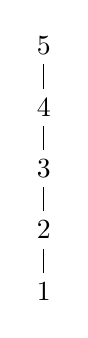
\begin{tikzpicture}[scale=0.6]
\node (1) at (0,0) {$1$};
\node (2) at (0,1.3) {$2$};
\node (3) at (0,2.6) {$3$};
\node (4) at (0,3.9) {$4$};
\node (5) at (0,5.2) {$5$};

\draw (1)--(2);
\draw (2)--(3);
\draw (3)--(4);
\draw (4)--(5);
\end{tikzpicture}
\end{center}

\end{frame}

\begin{frame}{Hasse Diagram of $(P(A),\subseteq)$}
Let

\[
A=\{1,2,3\}.
\]

Then

\[
P(A)=
\{\varnothing,\{1\},\{2\},\{3\},
\{1,2\},\{1,3\},\{2,3\},\{1,2,3\}\}.
\]

\begin{center}
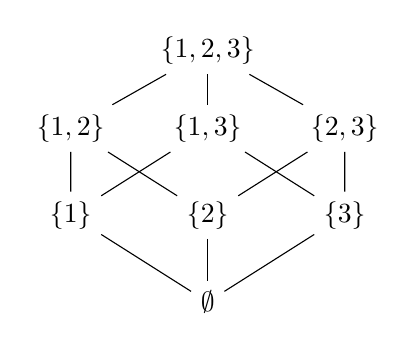
\begin{tikzpicture}[scale=0.58]
\node (123) at (0,5.5) {$\{1,2,3\}$};

\node (12) at (-3,3.8) {$\{1,2\}$};
\node (13) at (0,3.8) {$\{1,3\}$};
\node (23) at (3,3.8) {$\{2,3\}$};

\node (1) at (-3,1.9) {$\{1\}$};
\node (2) at (0,1.9) {$\{2\}$};
\node (3) at (3,1.9) {$\{3\}$};

\node (0) at (0,0) {$\emptyset$};

\draw (123)--(12);
\draw (123)--(13);
\draw (123)--(23);

\draw (12)--(1);
\draw (12)--(2);

\draw (13)--(1);
\draw (13)--(3);

\draw (23)--(2);
\draw (23)--(3);

\draw (1)--(0);
\draw (2)--(0);
\draw (3)--(0);
\end{tikzpicture}
\end{center}
\end{frame}


\begin{frame}{Inclusion--Exclusion Principle}
\begin{block}{Definition}
The Principle of Inclusion--Exclusion is used to find the number of elements in the union of overlapping finite sets.
\end{block}

For two finite sets $A$ and $B$,

\[
|A\cup B|
=
|A|+|B|-|A\cap B|.
\]

For three finite sets,

\[
\begin{aligned}
|A\cup B\cup C|
={}&|A|+|B|+|C|\\
&-|A\cap B|-|A\cap C|-|B\cap C|\\
&+|A\cap B\cap C|.
\end{aligned}
\]

The signs alternate between addition and subtraction.
\end{frame}

\begin{frame}{General Principle of Inclusion--Exclusion}
\small
\begin{block}{Theorem}
Let $A_1,A_2,\ldots,A_n$ be finite sets. Then
\end{block}

\[
\begin{aligned}
|A_1\cup A_2\cup\cdots\cup A_n|
={}&\sum |A_i|
-\sum |A_i\cap A_j|\\
&+\sum |A_i\cap A_j\cap A_k|
-\cdots\\
&+(-1)^{n+1}
|A_1\cap A_2\cap\cdots\cap A_n|.
\end{aligned}
\]

The pattern is

\[
+\text{single sets}
-\text{pairwise intersections}
+\text{three-way intersections}
-\cdots
\]
\end{frame}

\begin{frame}{Proof of the General Principle}
Suppose an element $x$ belongs to exactly $r$ of the given sets.

In the first summation, $x$ is counted once for each set containing it.

Hence, it is counted

\[
\binom{r}{1}
\]

times.

In the second summation, it is subtracted once for every pair of sets containing it.

Hence, it is subtracted

\[
\binom{r}{2}
\]

times.
\end{frame}

\begin{frame}{Proof: Continuing}
Similarly,

\[
+\binom{r}{3}
\]

is added from the three-set intersections,

\[
-\binom{r}{4}
\]

is subtracted from the four-set intersections, and so on.

Therefore, the total number of times $x$ is counted is

\[
\binom{r}{1}
-\binom{r}{2}
+\binom{r}{3}
-\cdots
+(-1)^{r+1}\binom{r}{r}.
\]
\end{frame}

\begin{frame}{Binomial Identity}
Using the binomial theorem,

\[
(1-1)^r=0.
\]

Therefore,

\[
\binom{r}{0}
-\binom{r}{1}
+\binom{r}{2}
-\cdots
+(-1)^r\binom{r}{r}=0.
\]

Since

\[
\binom{r}{0}=1,
\]

we obtain

\[
\boxed{
\binom{r}{1}
-\binom{r}{2}
+\binom{r}{3}
-\cdots
+(-1)^{r+1}\binom{r}{r}=1.
}
\]

Thus, each element is counted exactly once.
\end{frame}

\begin{frame}{Proof: Conclusion}
Since every element belonging to the union is counted exactly once,

\[
|A_1\cup A_2\cup\cdots\cup A_n|
\]

is equal to

\[
\sum |A_i|
-\sum |A_i\cap A_j|
+\sum |A_i\cap A_j\cap A_k|
-\cdots
\]

\[
+(-1)^{n+1}
|A_1\cap A_2\cap\cdots\cap A_n|.
\]

Hence,

\[
\boxed{\text{The General Principle of Inclusion--Exclusion is proved.}}
\]

\hfill$\blacksquare$
\end{frame}

\begin{frame}{AI/ML Example of Inclusion--Exclusion}
Suppose in an AI course:

\[
A=\{\text{students studying CNN}\},
\]

\[
B=\{\text{students studying RNN}\},
\]

\[
C=\{\text{students studying Transformers}\}.
\]

Suppose

\[
|A|=40,\qquad |B|=30,\qquad |C|=25,
\]

\[
|A\cap B|=10,\qquad
|A\cap C|=8,\qquad
|B\cap C|=7,
\]

and

\[
|A\cap B\cap C|=3.
\]
\end{frame}

\begin{frame}{AI/ML Example: Solution}
Using the three-set Inclusion--Exclusion formula,

\[
\begin{aligned}
|A\cup B\cup C|
={}&|A|+|B|+|C|\\
&-|A\cap B|-|A\cap C|-|B\cap C|\\
&+|A\cap B\cap C|.
\end{aligned}
\]

Substituting,

\[
|A\cup B\cup C|
=40+30+25-10-8-7+3.
\]

Therefore,

\[
\boxed{|A\cup B\cup C|=73}.
\]

Thus, 73 students study at least one of CNN, RNN or Transformers.
\end{frame}


\begin{frame}{Important Concepts: Summary}
\begin{itemize}
\item A set is a well-defined collection of distinct objects.
\item Set-builder form describes a set using a condition.
\item Roster form lists the elements explicitly.
\item Set operations include union, intersection, difference, symmetric difference, complement and Cartesian product.
\item A relation is a subset of a Cartesian product.
\item An equivalence relation is reflexive, symmetric and transitive.
\item A partial order is reflexive, antisymmetric and transitive.
\item A Hasse diagram represents a finite poset.
\item A chain contains comparable elements.
\item An antichain contains mutually incomparable elements.
\item Inclusion--Exclusion counts elements in overlapping sets.
\end{itemize}
\end{frame}

\begin{frame}{Thank You}
\begin{center}
\Huge\textbf{Thank You!}

\vspace{1cm}




\textbf{GAYATHRI P S}
\end{center}
\end{frame}

\end{document}
